%  !TeX  root  =  user_guide.tex

\chapter{Модули QGIS}\label{sec:plugins}\index{модули}

% when the revision of a section has been finalized,
% comment out the following line:
%\updatedisclaimer

Первоначально, QGIS был разработан на архитектуре с поддержкой различных
модулей, которые позволяют легко добавлять новые возможности или функции
в приложение. Большинство функций в QGIS осуществляются как
\textbf{основные} или \textbf{внешние} модули.\index{модули!виды}

\begin{itemize}[label=--]
\item \textbf{Основные модули} разрабатываются командой разработчиков
QGIS и автоматически входят в каждый новый релиз программы. Написаны они
либо на языках программирования C++ и Python. Более подробная информация
об основных модулях приведена в Разделе~\ref{sec:core_plugins}.
\item Все \textbf{Внешние модули} в настоящее время написаны на языке
Python. Они находятся во внешних репозиториях и поддерживаются
написавшими их авторами. Внешние модули могут быть добавлены с помощью
функции \filename{Установка модулей QGIS}. Более подробная информация
о внешних модулях приводится в Разделе~\ref{sec:external_plugins}.
\end{itemize}

\section{Управление модулями}\label{sec:managing_plugins}
\index{модули!управление}

Управление модулями подразумевает их загрузку или выгрузку с помощью
\filename{Менеджера модулей}. Внешние модули могут быть установлены,
активированы или удалены с помошью \filename{Загрузки модулей}.
Также \filename{Менеджер модулей} можно использовать для повторного
отключения/подключения внешних модулей.

\subsection{Загрузка основных модулей QGIS}\label{sec:load_core_plugin}

Загрузка основных модулей QGIS осуществляется из главного меню
\mainmenuopt{Модули} \arrow
\dropmenuopttwo{mActionShowPluginManager}{Управление модулями\ldots}.\index{модули!менеджер}

\begin{figure}[ht]
   \centering
   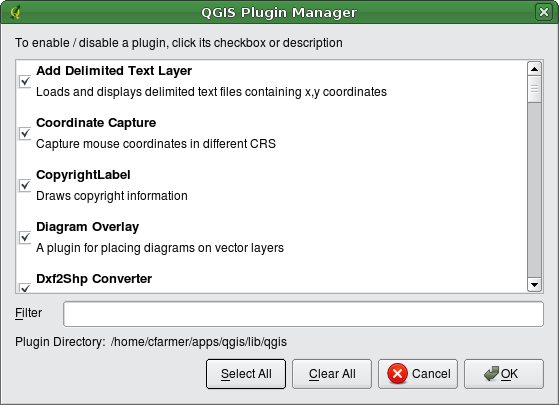
\includegraphics[clip=true, width=12cm]{pluginmanager}
   \caption{Менеджер модулей QGIS \wincaption}\label{fig:pluginmanager}\smallskip
\end{figure}

\filename{Менеджер модулей} содержит список всех доступных модулей,
включая основные и внешние, и их статус (загружен или нет).
Активируются модули автоматически с помощью установки флажка на соответствующем
модуле (см. Раздел~\ref{sec:external_plugins}).
На Рисунке~\ref{fig:pluginmanager} показано диалоговое окно Менеджера
модулей.

Для включения модуля достаточно установить флажок слева от его названия
и нажать кнопку \button{OK}. При выходе из приложения список
загруженных модулей сохраняется и будет автоматически загружен при
следующем запуске QGIS.

\begin{Tip}\caption{\textsc{Повреждённые модули}}\index{ошибки}
Если QGIS перестает загружаться, то, возможно, виноват повреждённый
модуль. Можно остановить загрузку модулей, отредактировав файл настройки
(см. Раздел~\ref{subsec:gui_options}). Найдите файл настроек модулей и
измените значение модулей на <<false>>, чтобы они не загружались при
запуске QGIS.
\nix {Например, чтобы прекратить загрузку модуля <<Текст с разделителями>>,
нужно отредактировать файл \$HOME/.config/QuantumGIS/qgis.conf
(в \nix) следующим образом:
\usertext{Add Delimited Text Layer=false}.}
\normalfont
Данное действие нужно повторить для каждого модуля в секции [Plugins].
После этого можно запускать QGIS, и через \filename{Менеджер модулей}
добавлять модули по одному, чтобы узнать, который из них является
причиной проблемы.
\end{Tip}

\subsection{Загрузка внеших модулей QGIS}\label{sec:load_external_plugin}

Для загрузки внешних модулей нужно выполнить всего один шаг:

\begin{itemize}[label=--]
\item Скачать модуль с внешнего репозиторя с помощью
\filename{Загрузки модулей} (Раздел \ref{sec:python_plugin_installer}).
Новый модуль будет добавлен в список доступных в
\filename{Менеджере модулей} и автоматически активирован.
\end{itemize}

\subsection{Использование менеджера модулей в QGIS}\index{модули!установка}\label{sec:python_plugin_installer}
\index{модули!Plugin Installer}\index{модули!обновление}

\begin{figure}[ht]
   \centering
   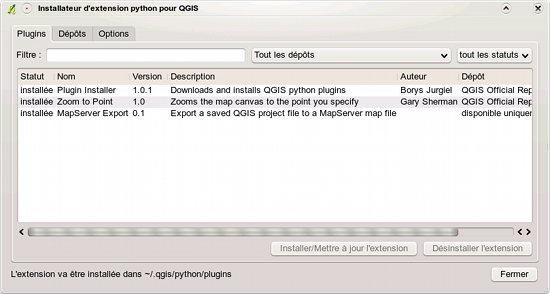
\includegraphics[clip=true, width=12cm]{plugininstaller}
   \caption{Установка модулей QGIS \wincaption}\label{fig:plugininstaller}\smallskip
\end{figure}

Для загрузки и установки внешних модулей нужно выбрать меню
\mainmenuopt{Модули} \arrow \dropmenuopttwo{plugin_installer}{Загрузить модули\ldots}.
Появится окно \filename{Установка модулей QGIS}
(рис.~\ref{fig:plugininstaller}) со вкладкой \tab{Модули}, в которой
отображается список всех установленных модулей, а также список доступных
для загрузки внешних модулей. Рядом с каждым модулем указан его статус:
\begin{itemize}[label=--]
\item \textbf{не установлен}"--- модуль доступен в репозитории, но еще
не загружен. Для установки нужно выбрать его и нажать кнопку
\button{Установить модуль}.
\item \textbf{новый}"--- новый модуль доступен в репозитории.
\item \textbf{установлен}"--- модуль уже установлен. Также будет
активна кнопка \button{Переустановить модуль}. Если доступна более
старая версия установленного плагина, то появится кнопка
\button{Понизить версию}.
\item \textbf{обновляемый}"--- модуль установлен, доступно обновление.
В этом случае будет активна кнопка \\
\button{Обновить модуль}.
\item \textbf{повреждён}"--- модуль установлен, но недоступен или
поврежден. Причина указана в описании к модулю.
\end{itemize}

\minisec{Вкладка Модули}

Для установки модуля необходимо выбрать его из списка и нажать кнопку
\button{Установить модуль}. Он будет активирован и установлен в
соответствующую директорию.

\begin{itemize}[label=--]
\item \nix{Linux и другие Unix-подобные системы}:\\
./share/qgis/python/plugins \\
/home/\$USERNAME/.qgis/python/plugins
\item \osx{Mac OS X}:\\
./Contents/MacOS/share/qgis/python/plugins \\
/Users/\$USERNAME/.qgis/python/plugins
\item \win{Windows}:\\
C:\textbackslash Program Files\textbackslash QGIS\textbackslash
python\textbackslash plugins \\
C:\textbackslash Documents and Settings\textbackslash\$USERNAME\textbackslash
.qgis\textbackslash python\textbackslash plugins
\end{itemize}

Если установка модуля прошла успешно, то появится соответствующее
сообщение.

Если при установке произошла ошибка, то ее причина будет указана в
отдельном окне на экране. Чаще всего ошибки возникают из-за проблем с
подключением нового модуля и/или отсутствием дополнительных модулей,
необходимых для работы нового модуля. В первом случае нужно немного
подождать перед повторным запуском установки. Во втором"--- установить
недостающие модули.
\nix{Для Linux, большинство модулей доступно через менеджер пакетов}.
\win{Для Windows"--- посетить домашнюю страницу модулей}.
Если используется прокси-сервер, нужно его настроить:
\mainmenuopt{Правка} \arrow \dropmenuopttwo{mActionOptions}{Параметры} (Gnome, OS\,X)
или \mainmenuopt{Настройки} \arrow \dropmenuopttwo{mActionOptions}{Параметры} (KDE, Windows)
вкладка \tab{Прокси} или \tab{Сетевые соединения}.

Кнопка \button{Удалить модуль} доступна для установленного модуля при
условии, что он не является основным. Обратите внимание, что если
включено обновление основных модулей, то можно удалить последнее
обновление кнопкой  \button{Удалить модуль} и вернуться к предыдущей
версии QGIS.

\minisec{Репозитории}

Вкладка \tab{Репозитории} содержит список источников для новых модулей.
По умолчанию включен только официальный репозиторий QGIS. Также можно
добавить и другие репозитории, воспользовавшись кнопкой
\button{Добавить сторонние репозитории}. Сторонние источники данных
содержат большое количество полезных модулей, но не поддерживаются
командой разработчиков QGIS. Также можно вручную управлять списком
репозиториев, добавляя, удаляя и редактируя записи. Временно отключить
репозиторий можно, нажав на кнопку \button{Изменить\ldots} и сняв флажок
в поле <<Активен>>.

\minisec{Параметры}

Вкладка \tab{Параметры} предназначена для настройки установки модулей.
Если установлен флажок \\
\checkbox{Проверять обновления при запуске}, то
при каждом включении QGIS он будет автоматически проверять наличие
новых и обновлённых модулей. По умолчанию, проверка будет происходить
из всех активных источников данных, которые указаны во вкладке
\tab{Репозитории}. Интервал проверки обновлений можно установить от
одного дня до месяца. Если будет доступен новый модуль или обновление
для установленного~--- появится соответствующее уведомление в строке
состояния. Если флажок автоматического обновления отключен, то проверка
будет происходить при каждом запуске \filename{Загрузки модулей} из
меню.

Если порт~80 закрыт, это может вызвать некоторые проблемы при
проверке обновлений. В этом случае, показатель
\textit{Поиск новых модулей\ldots} может отображаться в строке состояния
в течение всего времени работы с QGIS и может привести к ошибке при
попытке выхода из программы. Чтобы этого не произошло, небходимо
отключить автоматическую проверку обновлений при запуске программы.

Кроме того, можно указать тип модулей, которые будут отображатся в
\filename{Менеджере модулей}. В поле \textit{Разрешенные модули} можно
указать:

\begin{itemize}[label=--]
\item Показывать модули только из официального репозитория
\item Показывать все модули, кроме помеченных как экспериментальные
\item Показывать все модули, включая помеченные как экспериментальные.
\end{itemize}

\begin{Tip}
 \caption{\textsc{Использование экспериментальных модулей}}
Экспериментальные модули, как правило, непригодны для использования в
работе. Эти модули находятся на ранних стадиях разработки и могут
рассмотриваться как <<неполные>> или <<демонстрационные>>. Такие модули
не рекомендуется использовать в работе за исключением тестирования.
\end{Tip}

\section{Провайдеры данных}\index{провайдеры данных}

Провайдеры (поставщики) данных являются <<специальными>> модулями для
предоставления доступа к базам данных. По умолчанию, QGIS поддерживает
слои PostGIS и базы данных, основанных на библиотеках GDAL/OGR
(Приложение~\ref{appdx_ogr}). Эти модули позволяют расширить тип
поддерживаемых данных QGIS.

Модули провайдеров данных подключаются автоматически при каждом запуске
QGIS. Они не управляются из меню <<Управление модулями>> и включаются
тогда, когда слой добавлен в QGIS.

\FloatBarrier
